\chapter*{Introduction}
 The purpose of this project is to build an indoor WIFI-based positioning system. First of all, it is based on three different kinds of technologies : mobile phones (hosting an Android operation system), a computer (hosting a positioning server) and WIFI access points (TP-Link devices). \\
 \indent For this project, in order to be efficient, we had to divide the work to do into 3 categories, as mentioned above. Therefore, two persons were working on the server and the database, one working on the Android Application and finally one configuring the TP-Link devices. \\
 
\indent Considering how the positioning system works, one have to go through two main steps. The first one is called the calibration whose aim is to stock inside a database, some data that the mobile phone can send and which helps the server to locate afterwards the phone's position. The second step, called positioning, is used by the phone in order to be located in an indoor environment. \\
\indent The android application is what the user uses to perform the above-mentionned operations. It contains simple and intuitive graphical interfaces which are detailed in the user guide. \\
\indent Concerning the Access Points\footnote{Also known as AP}, we used OpenWRT and C langage. To be able to locate precisly an indoor device, we need to make measurements of the distance between the device and at least three points in the area. To do these measurements, we have implemented a solution which consists in measuring the strength of a signal emitted by the device which is captured by the APs. This is done by running a program on the TP-LINK's OS which sniffs packets flooding the network allowing to compute the RSSI of the device.\\
\indent The server can be considered as a link between the mobile phone, the TP-Link devices and the database. It communicates with each three of them and receive/send/insert/request data from/to entity.\\
\indent The tools we used to create this positioning system are, the Eclipse IDE in order to create the server, the different classes required for the project and to connect, through Hibernate to a postgreSQL database. We also used Android Studio to program the android application. \\ 
\indent We created a scheme to illustrate how our program works and the different interactions between the devices : \\

     \begin{figure}[H]
      \centering
      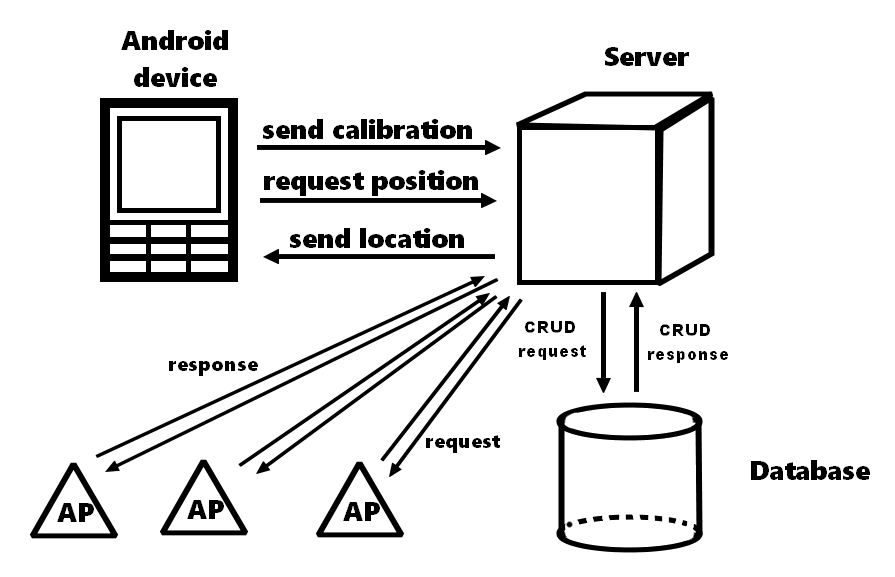
\includegraphics[scale = 0.50]{img/scheme_lo53_project.png}
      \caption{Overall communication scheme of the project.}
      \label{fig:overall_scheme}
     \end{figure}
  